%%%%%%%%%%%%%%%%%%%%%%%%%%%%%%%%%%%%%%%%%
% Journal Article
% LaTeX Template
% Version 2.0 (February 7, 2023)
%
% This template originates from:
% https://www.LaTeXTemplates.com
%
% Author:
% Vel (vel@latextemplates.com)
%
% License:
% CC BY-NC-SA 4.0 (https://creativecommons.org/licenses/by-nc-sa/4.0/)
%
% NOTE: The bibliography needs to be compiled using the biber engine.
%
%%%%%%%%%%%%%%%%%%%%%%%%%%%%%%%%%%%%%%%%%

%----------------------------------------------------------------------------------------
%	PACKAGES AND OTHER DOCUMENT CONFIGURATIONS
%----------------------------------------------------------------------------------------

\documentclass[
	a4paper, % Paper size, use either a4paper or letterpaper
	10pt, % Default font size, can also use 11pt or 12pt, although this is not recommended
	unnumberedsections, % Comment to enable section numbering
	twoside, % Two side traditional mode where headers and footers change between odd and even pages, comment this option to make them fixed
]{LTJournalArticle}

\addbibresource{references.bib} % BibLaTeX bibliography file

\usepackage{amsmath}

\runninghead{}

%\footertext{\textit{Journal of Biological Sampling} (2024) 12:533-684}
\footertext{}

\setcounter{page}{1}

%----------------------------------------------------------------------------------------
%	TITLE SECTION
%----------------------------------------------------------------------------------------

\title{Removing optimization problems' constraints\\ with two-step geometric transformations} 

% Authors are listed in a comma-separated list with superscript numbers indicating affiliations
% \thanks{} is used for any text that should be placed in a footnote on the first page, such as the corresponding author's email, journal acceptance dates, a copyright/license notice, keywords, etc
\author{%
	Oleksandr Kaleniuk\thanks{Corresponding author: \href{mailto:o.kaleniuk@kpi.ua}{o.kaleniuk@kpi.ua}}
}

% Affiliations are output in the \date{} command
\date{\footnotesize National Technical University of Ukraine "Igor Sikorsky Kyiv Polytechnic Institute"}

% Full-width abstract
\renewcommand{\maketitlehookd}{%
	\begin{abstract}
		\noindent From the geometric perspective, every continuous fragment of N-dimensional space constrained by strict inequalities is homeomorphic to the N-dimensional space itself. In this regard, every constrained optimization problem, where constraints are a set of inequalities, could be theoretically solved as a set of unconstrained problems.
		
For any practical purposes, however, applying an abstract transformation is not yet a method. Some of the most productive methods of numerical optimization rely on the differential properties of the target function, which might not survive the transformation. In this paper, we examine a two-step transformation that is not only continuous but also regular, allowing us to use Newtonian and quasi-Newtonian methods on the transformed target functions. The first step is the transformation from $\mathbb{R}^N$ to $[-1, 1]^N$. The second is the transformation from $[-1, 1]^N$ to either an N-dimensional linear hypercube mapping, an N-dimensional sphere, or an N-simplex. The list of second-step transformations can be continued, but this work only focuses on the three mentioned above.
	\end{abstract}
}

%----------------------------------------------------------------------------------------

\begin{document}

\maketitle % Output the title section

%----------------------------------------------------------------------------------------
%	ARTICLE CONTENTS
%----------------------------------------------------------------------------------------
\section{Problem statement}

Let's say we have a target $N$-ary function $T$ and a set of constraints $C$. The constrained space forms an inner space of either a hypercube, a simplex, or a unit sphere. We want to find a local optimum for the function $T$ within the constraints $C$ using a Newtonian or a quasi-Newtonian method of unconstrained optimization. For this, we want to define a transformation, or a composition of transformations $f g$, that maps $\mathbb{R}^N$ to $C$. The transformation $f(g(argopt_x T(f(g(x))))$ is the optimum of $T$ constrained in $C$.

\section{Literature review}

There are different approaches for turning an unconstrained optimization algorithm into a constrained one. The simplest approach would be to limit the type of constraints to per-coordinate boundaries. For instance, the implementation of the Nelder-Mead in the popular Python SciPy library keeps the simplex coordinates within the requested bounds by hard limiting their values \cite{Gao:2012}. 

Similar to that, the Bounded Optimization BY Quadratic Approximations (BOBYQA) \cite{Powell:2009} extends the unconstrained derivative-free optimization method NEWUOA \cite{Powell:2006} by introducing per-coordinate bounds.

The Constrained Optimization BY Linear Approximations (COBYLA) uses linear approximation of non-linear constraints and then applies a parametric penalty function to ensure that the approximation of the optimum found is adequately precise \cite{Powell:1994}.

The Constrained Optimization BY Quadratic Approximations (COBYQA) method allows both linear and non-linear constraints while using an optimization approach similar to bounded-only BOBYQA. COBYQUA way of constraint handling generalizes the Byrd-Omojokun approach \cite{Byrd:1987, Omojokun:1989} that allows defining equality constraints with inequality constraints \cite{Ragonneau:2022}. The method uses a parametric penalty function where the penalty parameter is variable. Using penalty functions is overall typical for the trust region-based optimization algorithms \cite{Conn:2000}. 

A similar approach could be used in the particle swarm optimization (PSO), although there are other methods typical for this class of optimization, namely bisection and preserving feasibility \cite{Innocente:2021}. However, a popular PSO library, Pyswarm, only allows per-coordinate bounds \cite{Miranda:2018}.

This paper proposes a different approach for turning a constrained optimization problem into an unconstrained one, and it involves mapping $\mathbb{R}^N$ onto the constrained area.

\section{Mappping $\mathbb{R}^N$ to $[-1, 1]^N$}

Let's presume we have a bounded optimization problem where $T(x, y)$ is the target function, and the boundaries are:

\begin{equation}
	\begin{array}{cc}
	x > -1 \\
	x < 1 \\
	y > -1 \\
	y < 1
	\end{array}
	\label{eq:boundaries}
\end{equation}

For example, if we define $T$ like this:
\begin{equation}
	T(x, y) = -3 cos(x - 0.1) + 2 cos(y + 2.2)
\end{equation}

Then the plot of this function and the constraints look like in figure \ref{fig:before1}. 

\begin{figure} 
	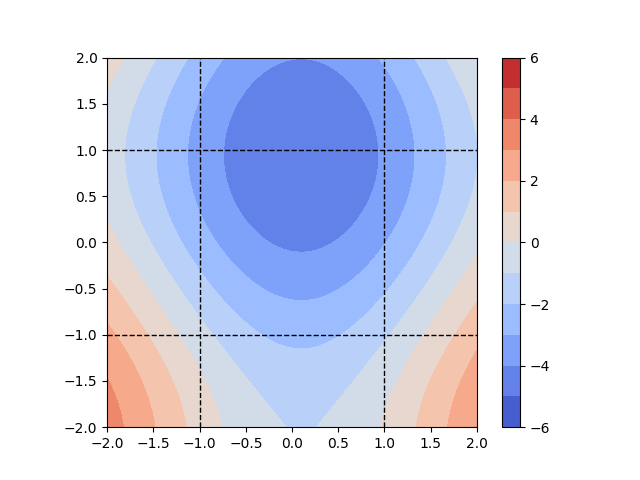
\includegraphics[width=\linewidth]{figure_1.png}
	\caption{An example of a bounded target function before any transformation}
	\label{fig:before1}
\end{figure}

The boundaries constrain the searching space for the optimization problem in a $[-1, 1]^2$ square. Let's introduce the transformation from $\mathbb{R}^N$ to $[-1, 1]^N$. One possible way to do so would be by using the arctangent function.

\begin{equation}
	f_i(x, y) = (\frac{arctan(x)}{\pi / 2}, \frac{arctan(y)}{\pi / 2})
	\label{eq:arctan_2d}
\end{equation}

Now the function $Ti(x,y) = T(f_i(x, y))$ is defined on the whole $\mathbb{R}^N$ but it only contains values from the $T(x, y)$ defined on the set of boundaries (\ref{eq:boundaries}). A plot of this function (now, of course, without constraints) is shown in figure \ref{fig:after_fi}. 

\begin{figure} 
	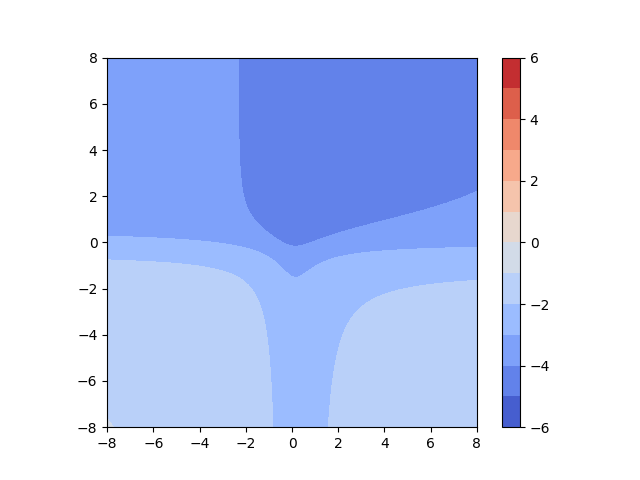
\includegraphics[width=\linewidth]{figure_2.png}
	\caption{An example of the unbounded target function after the arctangent transformation}
	\label{fig:after_fi}
\end{figure}

A solution of the unconstrained optimization problem on $T(f_i(x, y))$ will be equivalent to the solution of the bounded problem on $T(x, y)$ up to the transformation $f_i$. So given that the solution for the $T(f_i(x, y))$ is obtainable by any possible algorithm, and could be expressed as $x_i, y_i$, the equivalent solution for the $T(x, y)$ would be simply $f_i(x_i. y_i)$.

The transformation $f_i$ is continuous and regular. For the most part, it retains enough similarity with the original $T(x, y)$ function so that if a Newtonian or a quasi-Newtonian method was able to find a solution on unconstrained $T(x, y)$ within the bounded region, it would also be able to do so on the unbound $T(f_i(x, y))$. Near the boundaries, however, every function tends to degenerate into a plateau due to the nature of the arctangent transformation. So the iterative methods tend to converge very slowly.

Another possible way to remove the bounds for the $T(x, y)$ would be to use a periodic function such as sine.

\begin{equation}
	f_p(x, y) = (sin(x), sin(y))
	\label{eq:sine_2d}
\end{equation}

An example of a transformed function $T(f_p(x, y))$ is shown in figure \ref{fig:after_pi}. 

\begin{figure} 
	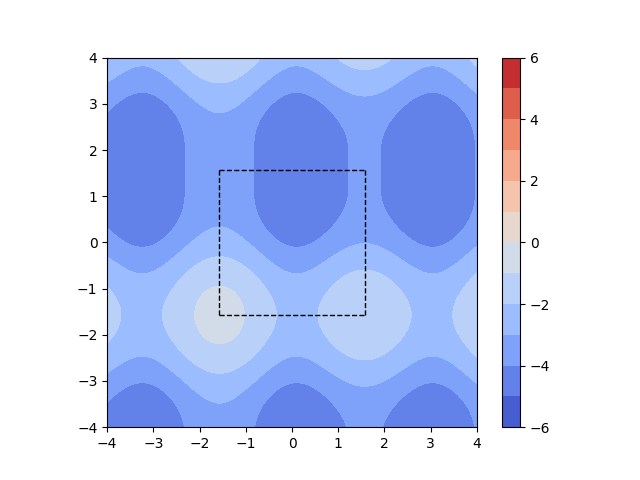
\includegraphics[width=\linewidth]{figure_3.png}
	\caption{An example of the unbounded target function after the sine transformation}
	\label{fig:after_pi}
\end{figure}

Such a transformation normally transforms a convex function into a non-convex one. A single optimum then becomes an infinite set of optimums. However, if there was one and only one local optimum in the bounded space, then all the optimums in the transformed space become equivalent under the $f_p$ transformation. Not only does this allow us to use Newtonian and quasi-Newtonian methods, but it also removes the complications with near-boundary solutions that were present with the arctangent transformation $f_i$.

\section{Mapping $[-1, 1]^N$ to $C$}

The cube $[-1, 1]^N$ can be transformed into a manifold of arbitrary shape. Let's call this transformation $g(x_1, x_2, ..., x_N)$. This means that if this manifold corresponds to the constraint space for optimization, the non-constrained method can be used to optimize a target function $T(x_1, x_2, ..., x_N)$ on the constraint space by using a combination of transformations $f$ from above and $g$. First we find the optimal point $x_uc = (x_{uc1}, x_{uc2}, ..., x_{ucN})$ in the unconstrained space $\mathbb{R}^N$, then we transform this point into the space the original $T$ is defined to get the optimal point $x_o$.

\begin{equation}
	\begin{array}{cc}
	x_{uc} = argopt T(g(f(x))) \\
	x_o = g(f(x_{uc}))
	\end{array}
	\label{eq:composition}
\end{equation}

In practice, we're not interested in abstract manifolds. We need a specific set of pragmatically applicable transformations with their differential properties known and their implications on the optimization problem-solving understood. This work proposes three such transformations:
\begin{enumerate}
  \item A transformation from $[-1, 1]^N$ to a linear transformation of a hypercube $[-1, 1]^N$.
  \item A transformation from $[-1, 1]^N$ to an N-simplex.
  \item And a transformation from $[-1, 1]^N$ to an N-dimensional sphere. 
\end{enumerate}

\subsection{Linear transformation of an N-hypercube}

Let's start from a 2-dimensional case. Let's say we have a target function $T(x, y)$, and a set of linear constraints that form some convex quadrilateral:

\begin{equation}
	\begin{array}{cc}
	y < a_1x+b_1 \\
	x < a_2y+b_2 \\
	y > a_3x+b_3 \\
	x > a_4y+b_4
	\end{array}
	\label{eq:linear_constraints}
\end{equation}

These constraints form a quadrilateral $C^2$:

\begin{equation}
	\begin{split}
    C^2 = ((x_{min1}, y_{min1}), (x_{min2}, y_{max2}),  \\ 
    (x_{max3}, y_{max3}), (x_{max4}, y_{min4}))
	\end{split}
	\label{eq:quadrilateral}
\end{equation}

An example of such rectangle constraining a target function is shown in figure \ref{fig:quadrilateral}.

\begin{figure} 
	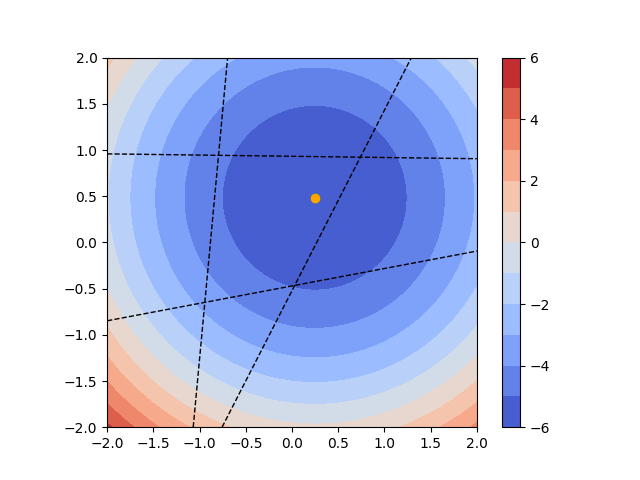
\includegraphics[width=\linewidth]{figure_4.png}
	\caption{An example of a binary target function constrained by a quadrilateral}
	\label{fig:quadrilateral}
\end{figure}

Let $g$ be a bilinear transformation.

\begin{equation}
	\begin{split}
	g(x, y) = (a_xxy+b_xy+c_xx+d_x, \\
	a_yxy+b_yy+c_yx+d_y)
	\end{split}
	\label{eq:bilinear_transformation}
\end{equation}

The inner space of the rectangle $[-1, 1]^2$ can then be transformed into the inner space of the quadrilateral $C^2$ in a way that:

\begin{equation}
	\begin{array}{cc}
	g(-1, -1) = (x_{min1}, y_{min1}) \\
	g(-1, +1) = (x_{min2}, y_{max2}) \\
	g(+1, +1) = (x_{max3}, y_{max3}) \\
	g(+1, -1) = (x_{max4}, y_{min4})
	\end{array}
	\label{eq:corners}
\end{equation}

This correspondence allows us to define 4 linear equations per every coordinate $x$ and $y$. Solving these equations will provide us with all the coefficients $a_x, b_x, c_x, d_x$ and $a_y, b_y, c_y, d_y$ respectively.

Let's define matrix $A$ as:
\begin{equation}
	\begin{bmatrix}
	+1 & -1 & -1 & +1 \\
	-1 & -1 & +1 & +1 \\
	+1 & +1 & +1 & +1 \\
	-1 & +1 & -1 & +1
	\end{bmatrix}
	\label{eq:corners_matrix}
\end{equation}

Now let's define vectors $B_x$ and $B_y$:

\begin{equation}
	\begin{array}{cc}
	B_x = [x_{min1}, x_{min2}, x_{max3}, x_{max4}] \\
	B_y = [y_{min1}, y_{max2}, y_{max3}, y_{min4}]
	\end{array}
	\label{eq:corners_vectors}
\end{equation}

Now solving these two equations will give us the coefficients for the $g$ transformation.

\begin{equation}
	\begin{array}{cc}
	A [a_x, b_x, c_x, d_x] = B_x \\
	A [a_y, b_y, c_y, d_y] = B_y
	\end{array}
	\label{eq:corners_equations}
\end{equation}

The transformation $g$ now transforms the space in a way that the inner space of the rectangle $[-1, 1]^2$ bijects the inner space of the quadrilateral $C^2$ but only if the quadrilateral is convex.

An example of such a bijection, that also transforms the function along with its optimum point, is shown in Figure \ref{fig:bilinear}.

\begin{figure} 
	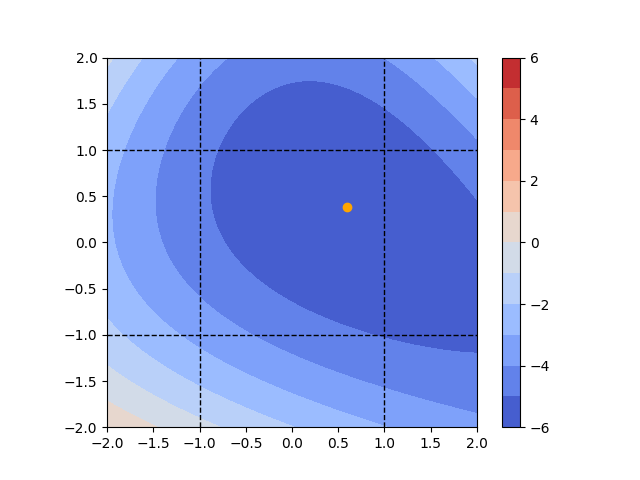
\includegraphics[width=\linewidth]{figure_5.png}
	\caption{An example of the bilinear transformation that makes a constrained optimization problem into a bounded one}
	\label{fig:bilinear}
\end{figure}

Now let $f$ be an arctangent transformation:

\begin{equation}
	\begin{split}
	f(x, y) = (\frac{arctan(x)}{\pi / 2}, \frac{arctan(y)}{\pi / 2})
	\end{split}
	\label{eq:arctangent_transformation}
\end{equation}

This transformation maps the whole $\mathbb{R}^2$ onto the inner space of $[-1, 1]^2$. The combination of transformations $f$ and $g$ transforms $\mathbb{R}^2$ onto the inner space of $C^2$. To optimize the target function constrained on $C^2$ we can now optimize the unconstrained function $T(f(g(x, y)))$, find the optimum point in the unconstrained space $x_{uc}$ and then transform the found optimum onto the $C^2$ with the same combination to find the true optimum point $x_o$ of the constraint target function $T$: $x_o = f(g(x_{uv}))$.

An example of a target function defined on the unconstrained space is shown in figure \ref{fig:unconstrained}.

\begin{figure} 
	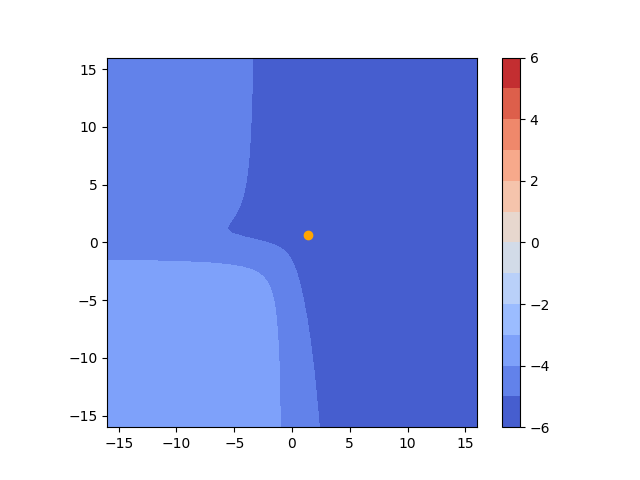
\includegraphics[width=\linewidth]{figure_6.png}
	\caption{An example of the target function mapped onto the unconstrained space}
	\label{fig:unconstrained}
\end{figure}

This approach generalizes fairly easily to $C^N$. The rectangle then becomes a linearly transformed hypercube; the coefficients of the $N$-dimensional linear transformations form a vector of $2^N$ elements, so the computational complexity of the transformation also rises exponentially. But the numeric values of the coefficients for the bilinear transformation are always deducible from the corners' coordinates of the bounding hypercube. And the coefficients of each corner point can easily be found by putting the corresponding linear equations that form the constraints into a linear system on $N$ equations and solving the system as we do when computing the planes' intersection.

For instance, the coordinates $(x_{min1}, x_{min2}, ..., x_{minN})$ can be found by gathering all the constraints of type $x_i > a_{i_N}*x_N + ... + a_{i_{i+1}}*x_{i+1} + a_{i_{i-1}}*x_{i-1} + ... + a_{i_2}*x_2 + a_{i_1}*x_1 + a_{i_0}$, where $a_{i_j}$ is the $j$-th coefficient of the $i$-th linear constraint, and making them into a system of linear equations:

\begin{equation}
	\begin{array}{cc}
a_{1_N}x_N + ... + a_{1_{i+1}}x_{i+1} - x_i + a_{1_{i-1}}x_{i-1} + \\ 
+ ... + a_{1_2}x_2 + a_{1_1}x_1 = -a_{1_0} \\
a_{2_N}x_N + ... + a_{2_{i+1}}x_{i+1} - x_i + a_{2_{i-1}}x_{i-1} + \\ 
+ ... + a_{2_2}x_2 + a_{2_1}x_1 = -a_{2_0} \\
... \\
a_{i_N}x_N + ... + a_{i_{i+1}}x_{i+1} - x_i + a_{i_{i-1}}x_{i-1} + \\ 
+ ... + a_{i_2}x_2 + a_{i_1}x_1 = -a_{i_0} \\
... \\
a_{1_N}x_N + ... + a_{N_{i+1}}x_{i+1} - x_i + a_{N_{i-1}}x_{i-1} + \\ 
+ ... + a_{N_2}x_2 + a_{N_1}x_1 = -a_{N_0} \\
	\end{array}
	\label{eq:nd_corner}
\end{equation}

Solving this system gives us the coordinates for one of the corners of the linearly transformed hypercube formed by the linear constraints. Solving $2^N$ such systems will give us enough values to form $N$ linear systems of $2^N$ equations that will represent the transformations of all the cube's corners. For the 2D, the corresponding equations are shown in formula (\ref{eq:corners_equations}).

Solving these equations will give us the coefficients for the transformation $g$. The transformation $f$ then remains almost the same as in formula (\ref{eq:arctangent_transformation}):

\begin{equation}
	\begin{split}
	f(x_1, x_2, ..., x_N) = (\frac{arctan(x_1)}{\pi / 2}, \frac{arctan(x_2)}{\pi / 2}, \\
	..., \frac{arctan(x_N)}{\pi / 2})
	\end{split}
	\label{eq:nd_arctangent_transformation}
\end{equation}

And the optimum point of the function $T$ constrained by $C^N$ could still be found by solving the unconstrained optimization problem on the transformed function as shown in formula (\ref{eq:composition}).

\subsection{N-simplex}
Simplices are used heavily in geometric modeling and finite element analysis. A triangle mesh representing a surface for 3D graphics is an example of a simplicial complex. A tetrahedral mesh of a 3D model prepared for FEA simulation is another. We can find an optimum of a function constrained by an $N$-dimensional simplex border using a principle similar to that we used for the hypercube constraints. Of course, we need another variant of the $g$ transformation.

Technically, there is no single best transformation from an $N$-simplex onto an $N$-dimensional cube $[-1, 1]^N$. There are at least $N!$ transformations that are equivalent for any pragmatical usage.

Let's look at the 2-dimensional example.

Let's say we have three linear constraints (\ref{eq:three_constaints}) that, while intersecting in pairs, define a triangle $ABC$ on the $\mathbb{R}^N$ plane as seen in figure \ref{fig:triangle_ABC}. We want to find the optimum of a function $T$ in the triangle $ABC$.

\begin{figure} 
	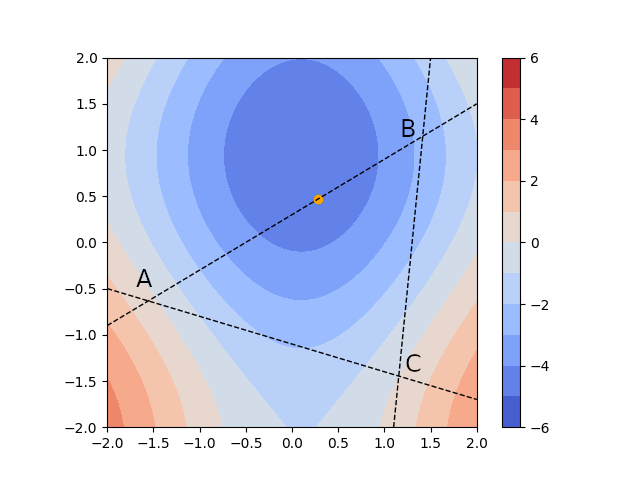
\includegraphics[width=\linewidth]{figure_7.png}
	\caption{An example of a target function constrained in a 2-simplex}
	\label{fig:triangle_ABC}
\end{figure}

\begin{equation}
	\begin{array}{cc}
x > a_1y + b_1 \\
y > a_2x + b_2 \\
y < a_3x + b_3 \\
	\end{array}
	\label{eq:three_constaints}
\end{equation}

The triangle's $ABC$ vertices appear where the lines representing the constraints intersect.

Let's $A$ be the intersecting points of the 1st and the 2nd constraint, $B$ - the 2nd and the 3rd, $C$ - the 3rd and the 1st. The specific coordinates of each point could then be obtained by solving 3 systems of 2 linear equations each.

\begin{equation}
	\begin{aligned} 
		\left\{ \begin{aligned} 
x_A - a_1y_A = b_1 \\
y_A - a_2x_A = b_2
		\end{aligned} \right. \\
		\left\{ \begin{aligned} 
y_B - a_2x_B = b_2 \\
y_B - a_3x_B = b_3
		\end{aligned} \right. \\	
		\left\{ \begin{aligned} 
y_C - a_3x_C = b_3 \\
x_C - a_1y_C = b_1
		\end{aligned} \right.
	\end{aligned}	
	\label{eq:ABC_systems}
\end{equation}

One way to define the $[-1, 1]^2$ to the 2-simplex transformation for the three vertices $A$, $B$, and $C$ would be this:

\begin{equation}
	\begin{split}
g(x, y) = \\
(x_A + (x_B-x_A)\frac{x+1}{2} + \\
(x_C-x_A)\frac{y+1}{2}(1-\frac{x+1}{2}),\\
y_A + (y_B-y_A)\frac{x+1}{2} + \\
(y_C-y_A)\frac{y+1}{2}(1-\frac{x+1}{2}))
	\end{split}
	\label{eq:ABC_transformation}
\end{equation}

Here the $\frac{x+1}{2}$ and $\frac{y+1}{2}$ transform $[-1, 1]^2$ into $[0, 1]^2$. Vectors $B-A$ and $C-A$ form a linear basis. The $[0, 1]^2$ square, if interpreted as coordinates in this basis, corresponds to the parallelogram that covers the simplex $ABC$ and an equivalent triangle we have no interest in. To limit $[0, 1]^2$ to the $ABC$ only, we multiply the second coordinate of the square by one minus the first coordinate. 

The formula (\ref{eq:ABC_transformation}) can be generalized onto a set of 6 transformations given that $A$, $B$, and $C$ are interchangeable. Not all of these 6 will be identical, but there is no good measure to assess the practical applicability of one transformation over another, so in this work, only the default transformation, the one described in (\ref{eq:ABC_transformation}) is further used.

An example of such a transformation transforming the $[-1, 1]^2$ to the triangle $ABC$ the target function from figure \ref{fig:triangle_ABC} is defined in is shown in figure \ref{fig:square_to_triangle_transformation}.

\begin{figure} 
	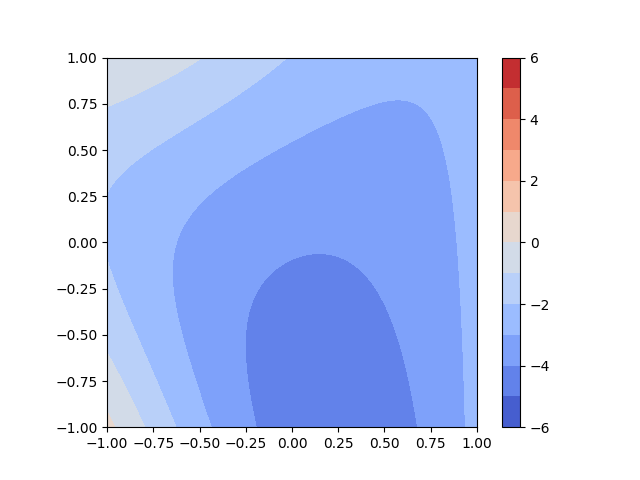
\includegraphics[width=\linewidth]{figure_8.png}
	\caption{An example of a square to triangle transformation applied to the target function from figure \ref{fig:triangle_ABC}}
	\label{fig:square_to_triangle_transformation}
\end{figure}

The formula (\ref{eq:ABC_transformation}) can be rewritten to clearly show that it is a special case of a bilinear transformation.

\begin{equation}
	\begin{split}
g(x, y) = \\	
(xy(\frac{x_A}{4}  - \frac{x_C}{4}) + x(\frac{-x_A}{4} + \frac{x_B}{2} - \frac{x_C}{4}) + \\
 y(\frac{-x_A}{4} + \frac{x_C}{4})  + \frac{x_A}{4} + \frac{x_B}{2} + \frac{x_C}{4}, \\
xy(\frac{y_A}{4}  - \frac{y_C}{4}) + x(\frac{-y_A}{4} + \frac{y_B}{2} - \frac{y_C}{4}) + \\
y(\frac{-y_A}{4} + \frac{y_C}{4})  + \frac{y_A}{4} + \frac{y_B}{2} + \frac{y_C}{4})
	\end{split}
	\label{eq:ABC_simpler_transformation}
\end{equation}

It can also be generalized to the N-dimensional case. Let's call the simplex vertices $v_i$ where $i = 1..N+1$. The coordinates of the point inside the cube $[-1, 1]^2$ will then be $x_j$ where $j = 1..N$, and the point itself $x = (x_1, x_2, ..., x_N)$. The formula (\ref{eq:ABC_transformation}) then becomes:

\begin{equation}
	\begin{split}
g(x) = \\
v_1 + \sum_{i=1}^{N} (v_{i+1} - v_1) \frac{x_i+1}{2}\prod_{j=1}^{i-1}(1-\frac{x_j+1}{2})
	\end{split}
	\label{eq:simplex_transformation}
\end{equation}

Note that while we were only referring to the constrained space and not the constraints themselves before while talking about the unconstraining transformation, with simplices it is possible, given their recurrent structure, to find an optimum not only in the N-simplex itself, but on its border too. This is possible because the border of an $N$-simplex is exactly $N+1$ $(N-1)$-simplices, which also have their borders as $N-2$-simplices, which in turn have their borders as $N-3$ simplices, etc. A 0-simplex is a point. So we can compute the target function in the simplex vertices, use unbounding transformations to find target function's optimums on the simplex edges, use similar transformations to find potential optimums on the simplex triangles, etc, until we have a set of potential optimums found on all possible borders of a given simplex. Then we can pick a minimum or a maximum with a simple discrete search.

Whether looking for the optimum recurrently in all N dimensions is practically applicable is questionable. Normally, the approximation of an optimum inside a simplex is good enough even if the true optimum lies exactly on the simplex border.

\subsection{N-dimensional sphere}

Once again, let's start from a 2-dimensional case. Let's say we have a spherical constraint $x^2+y^2 < 1$ and a function $T$ we want to find an optimum for in that sphere. The simplest way to make a transformation from a square $[-1, 1]^2$ to the sphere would be to linearly transform a pair of polar coordinates $r$ and $\phi$. An $r$ would correspond to the square's first coordinate, and the $\phi$ to the second.

\begin{equation}
	\begin{split}
g(x, y) = (\frac{x + 1}{2} cos(\pi y), \frac{x + 1}{2} sin(\pi y))
	\end{split}
	\label{eq:spherical_transformation1}
\end{equation}

This already enables us to use the composition (\ref{eq:composition}) and use unconstrained optimization to find the optimum constrained by the sphere. But for the spherical constraints, we can make the composition simpler if we choose our unbounding transformation $f$ to be periodic, such as (\ref{eq:sine_2d}).

\begin{equation}
	\begin{split}
fg(x, y) = (sin(x)sin(y), cos(x)sin(y))
	\end{split}
	\label{eq:spherical_transformation2}
\end{equation}

This function alone grants the transformation from $\mathbb{R}^2$ to the unit circle. The resulting function $T(fg(x, y))$ becomes periodic and loses the convex property if it has been convex before (as in figure \ref{fig:circular_constrained}) but with this transformation, most of the unconstrained optimization algorithms are still able to find the optimum on the source function $T$ because, firstly, the transformation itself is regular so it doesn't prohibit differentiation anywhere enabling Newtonian and quasi-Newtonian methods to work, secondly, even if the function $T(fg(x, y))$ has the infinite amount of optimal points, they are all equal, and they all correspond to the single point in the constrained space under the same transformation $fg$. 

You can see this in figure \ref{fig:circular_unconstrained}: the inner space of the circle corresponds to the square marked with a dashed line in the figure, but the rest of the function is a repeated pattern everywhere on $\mathbb{R}^2$.

\begin{figure} 
	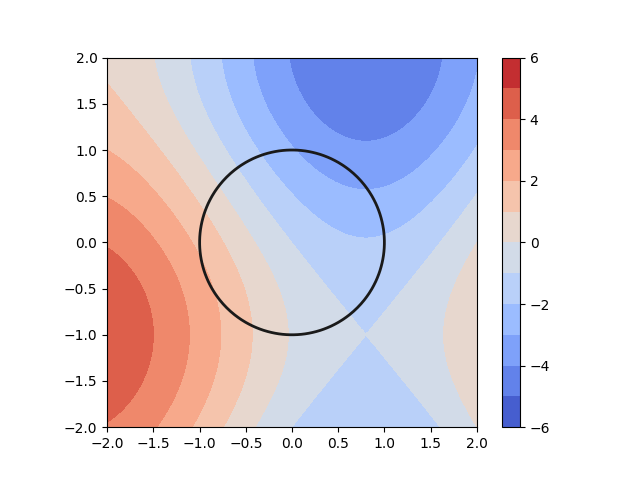
\includegraphics[width=\linewidth]{figure_9.png}
	\caption{An example of a function constrained within a unit circle}
	\label{fig:circular_constrained}
\end{figure}

\begin{figure} 
	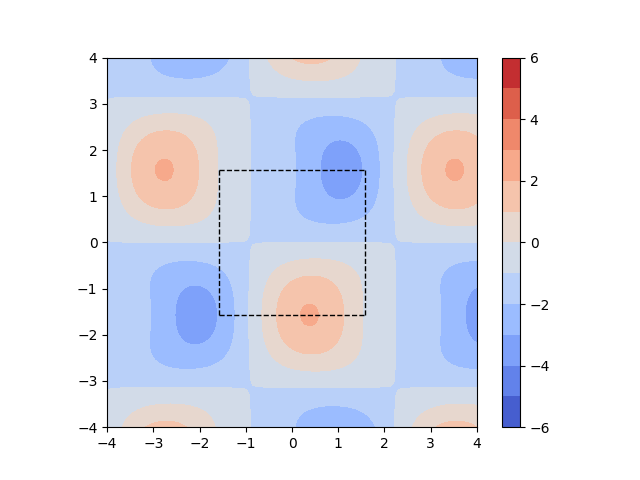
\includegraphics[width=\linewidth]{figure_10.png}
	\caption{An example of a function being "unconstrained" by a periodic transformation}
	\label{fig:circular_unconstrained}
\end{figure}

%------------------------------------------------

\section{Experiments}

To explore the practical applicability of the proposed method, a series of computational experiments were conducted. Each series was dedicated to a particular combination of transformations:
\begin{enumerate}
  \item The arctangent transformation from $\mathbb{R}^2$ to $[-1, 1]^2$ (\ref{eq:arctan_2d}) combined with the transformation from $[-1, 1]^2$ to a bilinear transformation of a square (\ref{eq:bilinear_transformation}) to minimize a quadratic function with 4 linear constraints.
  \item The periodic transformation from $\mathbb{R}^2$ to $[-1, 1]^2$ (\ref{eq:sine_2d}) combined with the transformation from $[-1, 1]^2$ to a bilinear transformation of a square (\ref{eq:bilinear_transformation}) to minimize a quadratic function with 4 linear constraints.
  \item The arctangent transformation from $\mathbb{R}^2$ to $[-1, 1]^2$ (\ref{eq:arctan_2d}) combined with the transformation from $[-1, 1]^2$ to a 2-simplex (\ref{eq:ABC_transformation}) to minimize a quadratic function with 3 linear constraints.
  \item The periodic transformation from $\mathbb{R}^2$ to $[-1, 1]^2$ (\ref{eq:sine_2d}) combined with the transformation from $[-1, 1]^2$ to a 2-simplex (\ref{eq:ABC_transformation}) to minimize a quadratic function with 3 linear constraints.
  \item The bi-periodic transformation from $\mathbb{R}^2$ to a unit circle (\ref{eq:spherical_transformation2}) to minimize a quadratic function on a unit circle.
\end{enumerate}

The target function for all series was made to have a random minimum in the $(-1, 1)^2$ square's inner space.

For the first 4 series, the initial configuration of constraints had been randomized along with the target function. 

For the first 2 series, the initial constraints were given by four points of their intersections. The points were randomly generated in $(-1, 0)^2$, $(-1, 0)\times(0, 1)$, $(0, 1)^2$, and $(0, 1)\times(-1, 0)$ squares. In this way, the linear constraints always form a convex quadrilateral, which is a necessary condition for the bilinear transformation.

For series 3 and 4, the constraints were given by the three points of intersection randomized in: $(-1, 0)\times(-0.5, 0.5)$, $(0, 1)^2$, and $(0, 1)\times(-1, 0)$. 

The experiments concluded compared relative effectiveness of COBYLA with constraints \cite{Powell:1994} and unconstrained BFGS \cite{fletcher:1987} on transformed target functions. The main factor that was considered as a measure of effectiveness was the number of target function evaluation.

The experiments have shown that BFGS with arctangent transformation $f$ (\ref{eq:arctan_2d}) usually loses in performance to COBYLA if the minimum points lies outside the constraints. It is also observed that the chance of BFGS outperforming COBYLA goes down as the minimum point gets closer to the constraints even while technically staying inside. This may be attributed to the nature of arctangent transformation that creates quasi-plateau near the constraints as the space within contraints gets transformed disproportionately: a small translation in the origin space of the target function corresponds to the larger and larger translation in the $\mathbb{R}^N$ space as the point in question approaches the constraints. 

This effect is observable both for the square (\ref{eq:bilinear_transformation}) and 2-simplex (\ref{eq:ABC_transformation}) transformations $g$. 

With the periodic transformation (\ref{eq:sine_2d}) and bilinear transformation (\ref{eq:bilinear_transformation}), BFGS outperforms COBYLA in roughly 2/3 of all the test runs. However, it is worth noticing that the total amount of target function evaluations differs between algorithms by less than 10\%, so the difference in pragmatic efficiency seems negligible.

With the periodic transformation (\ref{eq:sine_2d}) and 2-simplex transformation (\ref{eq:bilinear_transformation}), BFGS outperforms COBYLA in about 1/2 of all the test runs. The total amount of target function evaluations is 10\%-20\% more for BFGS, so COBYLA shows slightly more performant.

With the bi-periodic transformation (\ref{eq:spherical_transformation2}) to the unit circle, BFGS outperforms COBYLA in about 2/3 of all the run cases. The difference in total function evaluation counts is about 10\% in favor of BFGS.

Regarding the precision, BFGS with the bi-periodic transformation has the upper hand when the randomized minimum lies outside the unit circle, not in. BFGS gives a better approximation in about 99\% of all the test runs; however, the difference in total error between the two algorithms is negligible. In 1024 test runs, the difference in total error is only about 1e-4.

Considering all the evidence, BFGS with the proposed transformation gives a small performance and precision boost in some of the problems explored. However, the scale of improvement doesn't seem to be game changing for any practical problem.

The source code for all the experiments is available on GitHub: \url{https://github.com/akalenuk/unconstraining_transformations}.
%------------------------------------------------

\section{Discussion}

The proposed method may not show any drastic improvement over existing algorithms on lightweight target functions and primitive constraint configurations we examined. But the experimental results show promise, especially regarding the non-linear constraints. It is worth noticing that while the traditional approach segregates linear and non-linear constraints, for the transformation-based approach, any transformation that maps $\mathbb{R}^N$ to any constrained area is inherently non-linear, so there is no difference whether the constraints themselves are linear or not.

Effectively, this enables employing non-linear transformations from $[-1, 1]^N$ to the constrained area. We have already seen one in the context of cube to sphere transformation (\ref{eq:spherical_transformation2}), but we can also use quadratic or cubic transformations for handling quadratic or cubic constraints, respectively.

There is also space for improvement regarding setting constraints in polar coordinates. So far, we only looked at the unit circle; however, it is easy to generalize the approach for optimizing a target function constrained by another function $c$ in polar coordinates so that $c: \phi \rightarrow r$. An example of solving such an optimization problem is shown in Figure \ref{fig:polar_constrained}.

\begin{figure} 
	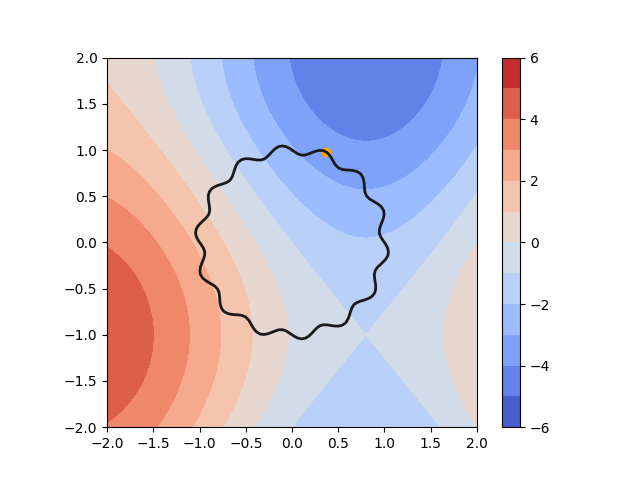
\includegraphics[width=\linewidth]{figure_11.png}
	\caption{A constraint given as a sinusoidal function in polar coordinates}
	\label{fig:polar_constrained}
\end{figure}

Solving this problem with a traditional approach would be difficult. The computational complexity of the linear approximation of a sinusoid in polar coordinates depends on its period, while the computational complexity of a bi-periodic transformation doesn't.

There might also be problems where there is already a mapping function we can use as the transformation from a unit cube to the constrained space. For instance, if we want to minimize something on a surface given as a spline patch. In this case, the natural parameterization of the spline is already a mapping function we can use as an $g$ part of the $fg$ transformation.

It would be interesting to investigate such problems in the future, but that goes beyond the scope of this particular paper.

\section{Conclusions}

This paper proposes an approach to solve optimization problems with constraints by mapping the $\mathbb{R}^N$ onto the constrained area and solving the unconstrained optimization problem on that map. To make the approach modular, the transformation is split into a 2-step transformation. First the $\mathbb{R}^N$ to $[-1, 1]^N$ transformation, then the $[-1, 1]^N$ to the constrained area. In this paper, two transformations of the former type and three of the latter are examined.

The experiments show that the proposed approach offers little to no benefit in solving problems of mathematical optimization with constraints compared to other well-established methods. There are small gains in terms of performance and precision that it can provide in one context or another, but the scale of these benefits is small. However, the general approach is also applicable to problems that would be hard to tackle with more traditional methods.


%----------------------------------------------------------------------------------------
%	 REFERENCES
%----------------------------------------------------------------------------------------

\printbibliography % Output the bibliography

%----------------------------------------------------------------------------------------

\end{document}
